\chapter{Preparation}
\section{The Mach-Zehnder Modulator}
\begin{figure}
  \centering
  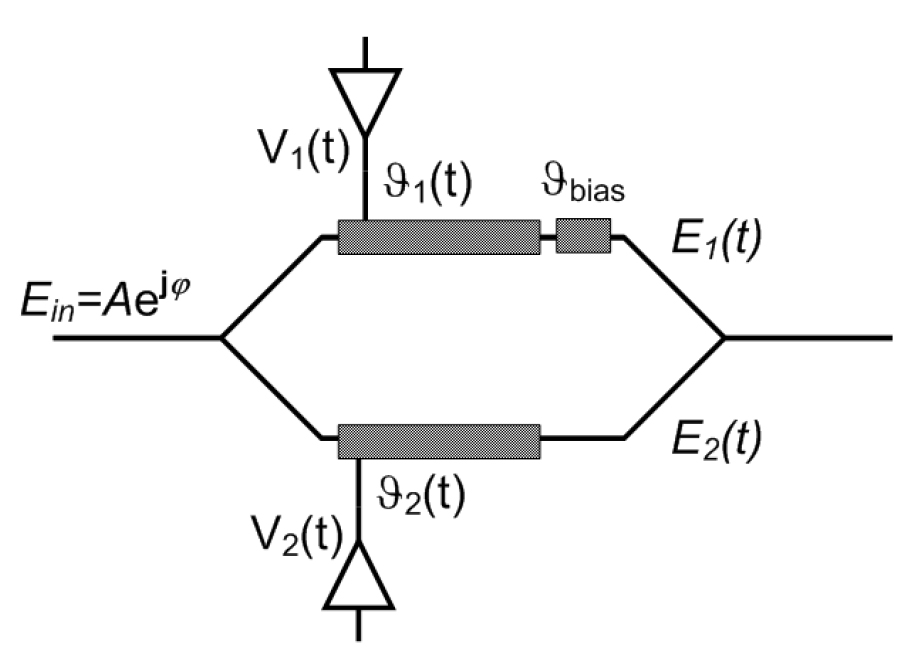
\includegraphics[width=.5\columnwidth]{Grafiken/Mach-Zehnder.jpg}

\caption{}
\label{fig:MZI}
\end{figure}
In a Mach-Zehnder Modulator the light is split up in two branches. In each branch there is a non-linear medium, through which the Phase of the Light can be shifted. At the end the Light is brought together, so that it is interfering. This setup is shown in fig. \ref{fig:MZI}. The Amplitude of the Field at the end of the Modulator can be expressed as:
\begin{equation}
 E_{\mathrm{out}}=\exp\left(j\frac{\vartheta_1+\vartheta_2}{2}+j\frac{\vartheta_{\mathrm{Bias}}}{2} \right)\cdot\cos\left(\frac{\vartheta_1-\vartheta_2}{2}+\frac{\vartheta_{\mathrm{Bias}}}{2}\right)\cdot E_{\mathrm{in}} .
\end{equation}
The phase shift of the Signal at the output of the modulator is described by the first term, the amplitude by the second term. For the phase Modulation $\vartheta_1 = \vartheta_2$ only the phase of the Signal is changed while the Amplitude stays constant. This operation mode is called "`push-push"' mode. For $\vartheta_1 = -\vartheta_2$ only the Amplitude of the Signal is modulated. This operation mode is called "`push-pull"' mode. \todo{Null-point vs. quadrature point} \cite{OCS}

\begin{figure}
  \centering
  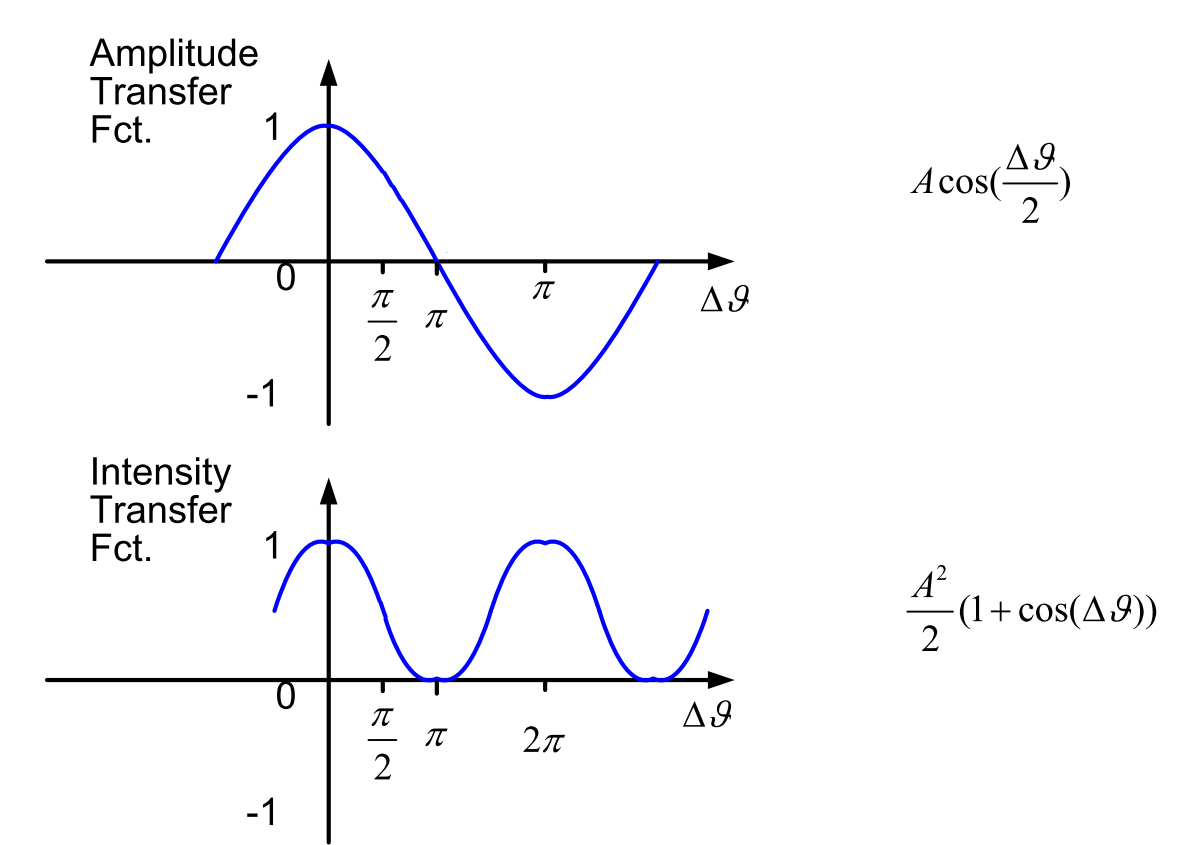
\includegraphics[width=.5\columnwidth]{Grafiken/Mach-Zender-Transfer.jpg}

\caption{}
\label{fig:MZI_plot}
\end{figure}


\section{Modulation Formats}
\subsection{Amplitude Shift Keying}
In Amplitude Shift Keying (AFK) information is transmitted trough the signal amplitude. The level of the signal amplitude defines a binary value. There is the case "On/Off keying" (OOK) where the binary symbol is "0" when there is no power transmitted. It's a "1" when there is power transmitted. 
Figure \ref{fig:ask} shows such an ASK signal.

\begin{figure}
  \centering
  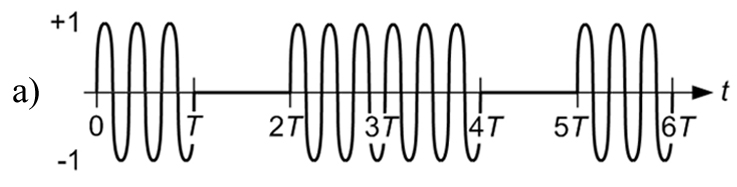
\includegraphics[width=.5\columnwidth]{Grafiken/OOK.jpg}
	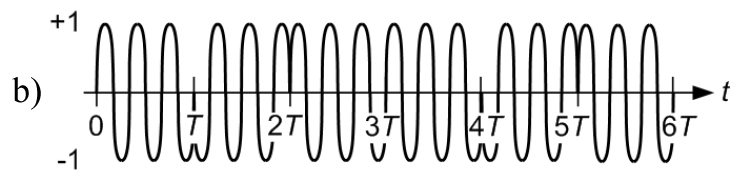
\includegraphics[width=.5\columnwidth]{Grafiken/PSK.jpg}%
\caption{\textbf{a)} Amplitude Shift Keying \textbf{b)} Phase Shift Keying}
\label{fig:ask}
\end{figure}



\subsection{Quadrature Amplitude Modulation}


\section{Signal Generation}

\section{RZ Signal Generation}